\documentclass{beamer}
\usepackage{ctex, hyperref}
\usepackage[T1]{fontenc}

% other packages
\usepackage{latexsym,amsmath,xcolor,multicol,booktabs,calligra}
\usepackage{graphicx,pstricks,listings,stackengine,adjustbox}
\usepackage{ctex, hyperref}
\usepackage{tikz,algorithm,algorithmic}
\usepackage{animate}

\author{李明睿}
\title{深度强化学习}
\institute{北京航空航天大学}
\date{2026年04月14日}
\usepackage{Buaa}

% defs
\def\cmd#1{\texttt{\color{red}\footnotesize $\backslash$#1}}
\def\env#1{\texttt{\color{blue}\footnotesize #1}}
\definecolor{deepblue}{rgb}{0,0,0.5}
\definecolor{deepred}{rgb}{0.6,0,0}
\definecolor{deepgreen}{rgb}{0,0.5,0}
\definecolor{halfgray}{gray}{0.55}

\lstset{
    basicstyle=\ttfamily\small,
    keywordstyle=\bfseries\color{deepblue},
    emphstyle=\ttfamily\color{deepred},    % Custom highlighting style
    stringstyle=\color{deepgreen},
    numbers=left,
    numberstyle=\small\color{halfgray},
    rulesepcolor=\color{red!20!green!20!blue!20},
    frame=shadowbox,
}


\begin{document}

\kaishu
\begin{frame}
    \titlepage
    \begin{figure}[htpb]
        \begin{center}
            
\includegraphics[width=0.2\linewidth]{pic/buaa_log.eps}
        \end{center}
    \end{figure}
\end{frame}

\begin{frame}
    \tableofcontents[sectionstyle=show,subsectionstyle=show/shaded/hide,subsubsectionstyle=show/shaded/hide]
\end{frame}

\begin{frame}{什么是强化学习？}
\begin{columns}[T]
    \begin{column}{0.55\textwidth}
        \begin{block}{核心问题}
            智能体（Agent）如何通过与环境（Environment）交互，学习一套使长期累积奖励最大的决策策略？
        \end{block}
        \textbf{关键元素：}
        \begin{itemize}
            \item 状态 $s_t$：环境在时刻 $t$ 的观测
            \item 动作 $a_t$：智能体采取的决策
            \item 奖励 $r_t$：环境给出的即时反馈
            \item 策略 $\pi(a|s)$：从状态到动作的映射
            \item 回报 $G_t = \sum_{k=t}^{T} \gamma^{k-t} r_k$
        \end{itemize}
        {\small 强化学习优化的是\textbf{长期回报}，不是单步最优。}
    \end{column}
    \begin{column}{0.42\textwidth}
        \centering
        \includegraphics[width=0.4\linewidth]{}
        \begin{block}{MDP五元组}
            \[
            (\mathcal{S}, \mathcal{A}, P, R, \gamma)
            \]
        \end{block}
    \end{column}
\end{columns}
\end{frame}

\begin{frame}{强化学习的本质}
    收集信息，探索信息，决定优化方向

    深度学习是数据的学科
\end{frame}

\section{发展历史与研究现状}

\begin{frame}{动态规划}
    % --- 使用columns环境实现左右分栏 ---
\begin{columns}[T]  % [T] = 顶部对齐（Top），可选[c]居中、[b]底部

    % ===== 左栏：文字介绍（占60%宽度）=====
    \begin{column}{0.6\textwidth}        
        % 大标题
        {\Large \textbf{Richard Bellman}}\\
        \vspace{0.2cm}
        {\small (1920–1984)}
        % 时间标注
        \begin{block}{1957年：里程碑}
            发表动态规划理论，提出\textbf{Bellman方程：}
        \end{block}
        $\begin{gathered}
        V(s) = \max_{a} \big[ R(s,a) + \gamma \sum_{s'} P(s'|s,a)V(s') \big]
        \end{gathered}$
        
        \vspace{0.1cm}

         \begin{itemize}
            \item 将多阶段决策问题分解为子问题
            \item 提出\textbf{最优性原理}：
                  \begin{quote}
                  \small "一个最优策略的子策略必须是最优的"
                  \end{quote}
            \item 为强化学习奠定数学基础
        \end{itemize}


    \end{column}
     % ===== 右栏：照片（占35%宽度，留5%间隙）=====
    \begin{column}{0.35\textwidth}
        \centering
        
        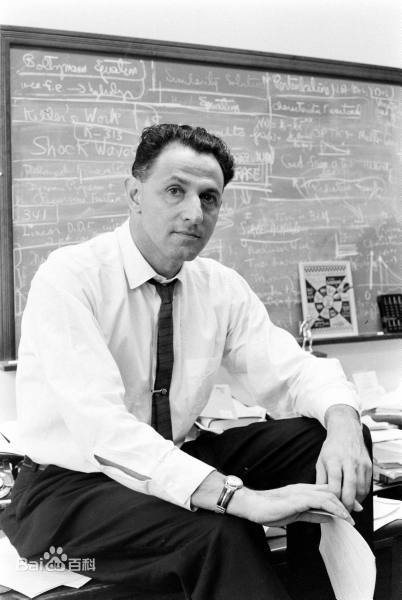
\includegraphics[width=\textwidth]{bellman.jpeg}
        
        % 照片说明
        {\small Richard Bellman\\
        美国应用数学家\\
        {\color{purple}{动态规划}}之父}
    \end{column}

\end{columns}
\end{frame}

 \begin{frame}{强化学习书目推荐}
      % 左侧：照片和简介
      \begin{columns}
          \begin{column}{0.5\textwidth}
              \centering
              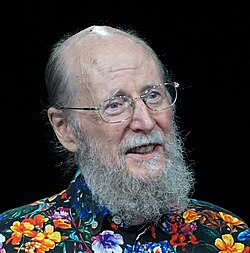
\includegraphics[width=0.7\linewidth]{images/Richard_S.jpg}\\
              \vspace{0.1cm}
              \textbf{Richard S. Sutton}\\
              \small{强化学习之父}\\
              \vspace{0.1cm}
              \tiny{
              \begin{itemize}
                  \item 加拿大计算机科学家，阿尔伯塔大学教授
                  \item 2024年图灵奖得主（与Andrew Barto共同获得）
                  \item 时间差分学习（TD Learning）发明者
                  \item 发表论文被引用约17万次
              \end{itemize}
              }
          \end{column}

          % 右侧：书籍封面
          \begin{column}{0.5\textwidth}
              \centering
              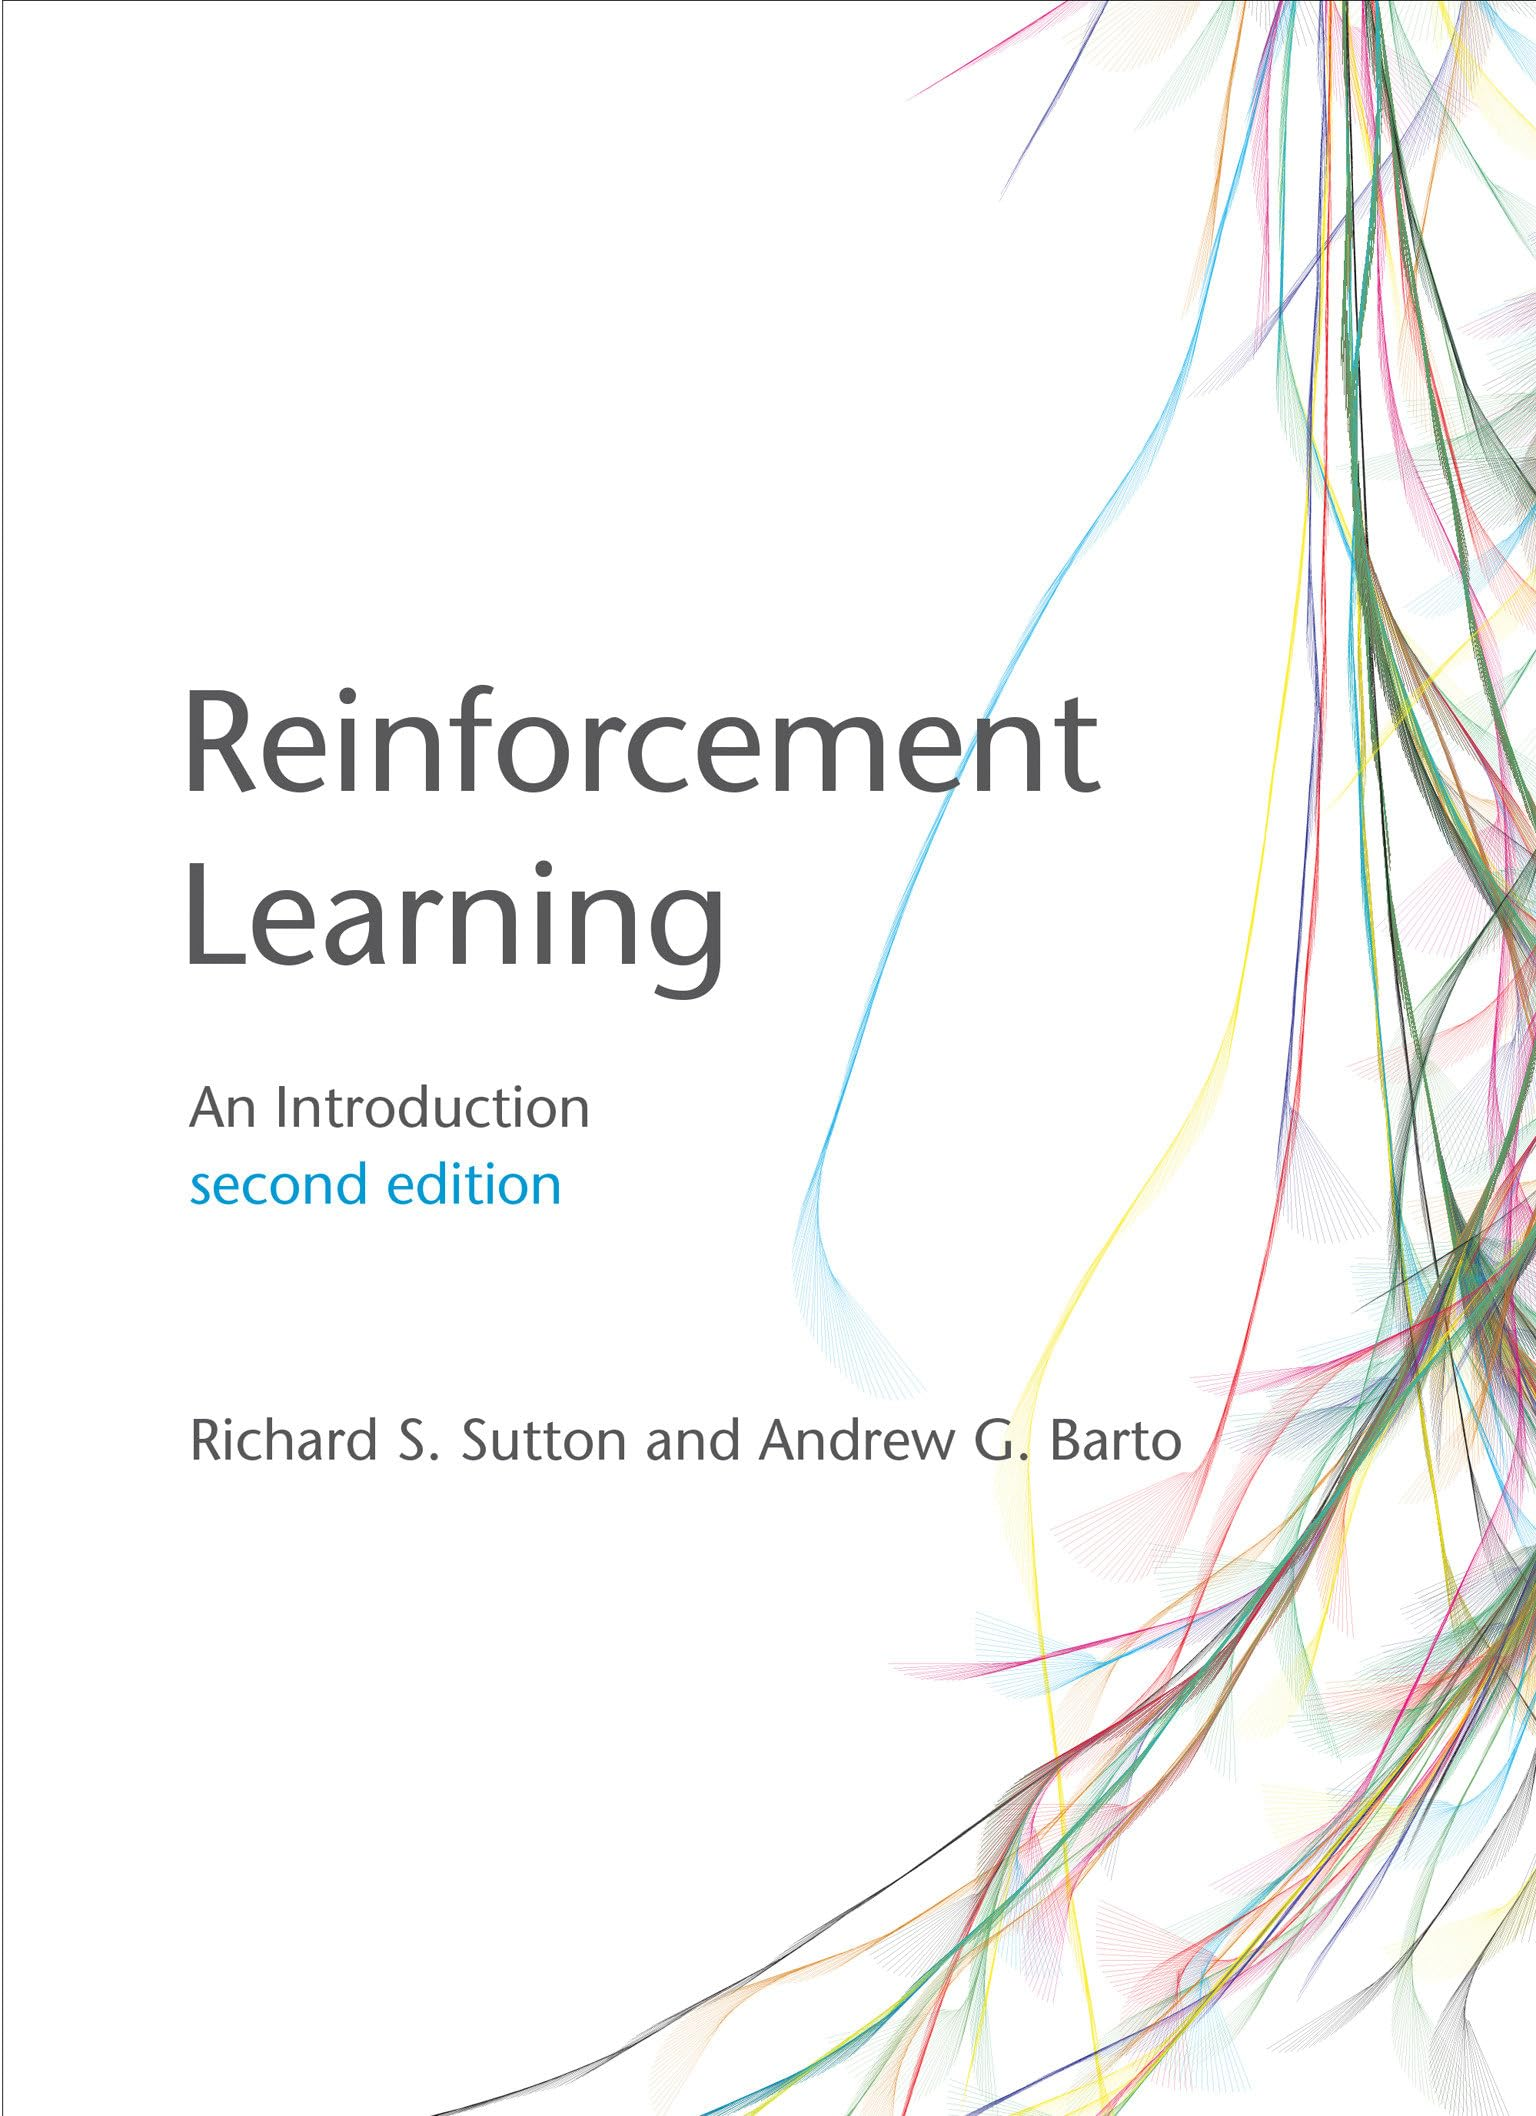
\includegraphics[width=0.6\linewidth]{images/RLbook_cover.jpg}
              \vspace{0.3cm}
              \small{
              \textbf{Reinforcement Learning: An Introduction}
              \cite{Reinforcement_Learning}}
          \end{column}
      \end{columns}
  \end{frame}

\begin{frame}{强化学习书目推荐}
      \begin{columns}[T]  % [T] 表示顶部对齐
          % 左侧
          \begin{column}{0.5\textwidth}
              \centering
              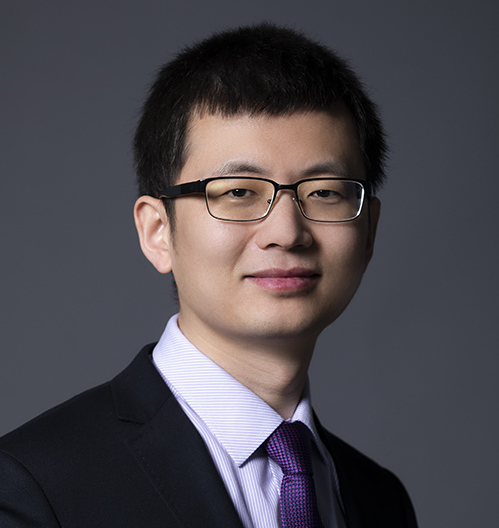
\includegraphics[width=0.6\linewidth]{images/zhaoshiyu.jpg}\\
              \vspace{0.2cm}
              \textbf{赵世钰 教授}\\
              \small{西湖大学工学院}
          \end{column}

          % 右侧
          \begin{column}{0.5\textwidth}
              \centering
              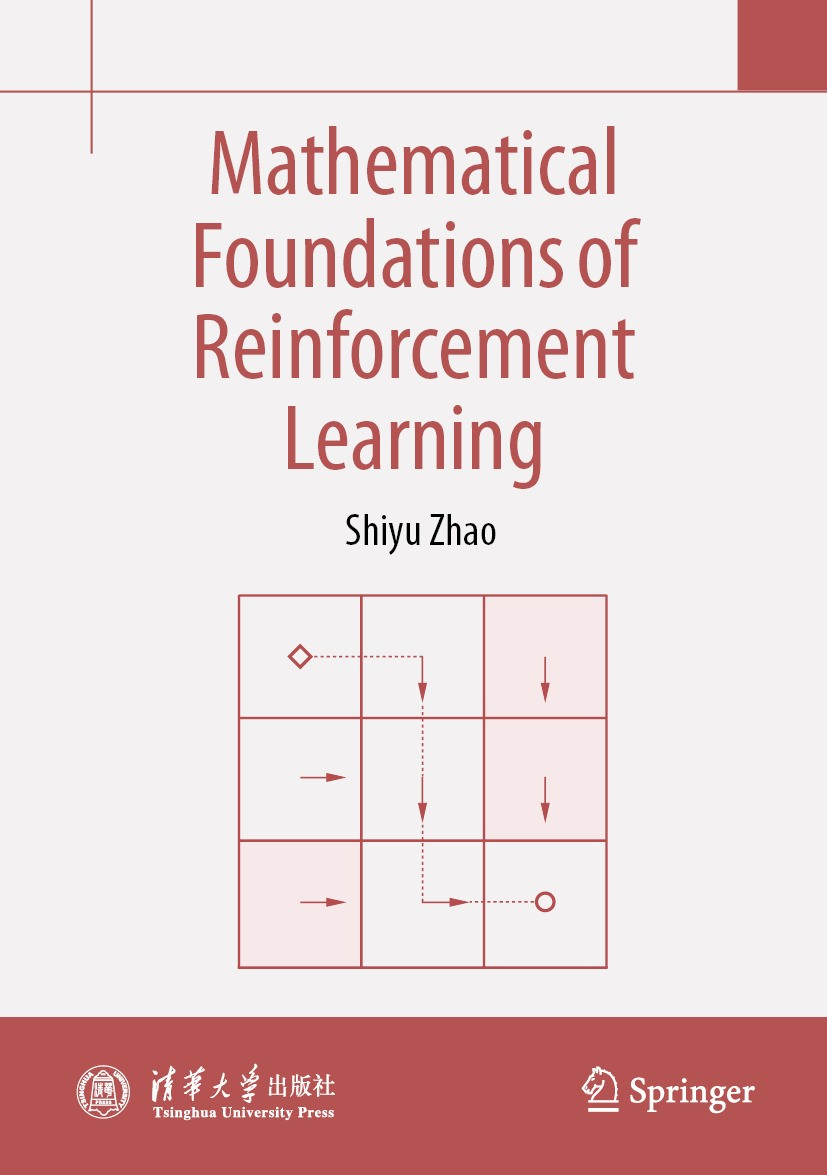
\includegraphics[width=0.5\linewidth]{images/MathRL.jpeg}\\
              \vspace{0.2cm}
              \textbf{《强化学习的数学原理》}\\
              \vspace{0.1cm}
              \small{
                  \begin{itemize}
                      \item 理论扎实，推导清晰
                      \item 配套视频课程
                      \item 中文强化学习入门首选
                  \end{itemize}
              }
          \end{column}
      \end{columns}
  \end{frame}

\begin{frame}[强化学习(RL)在Atari游戏中的应用]
\begin{columns}[T]
    \begin{column}{0.48\textwidth}
        \centering
        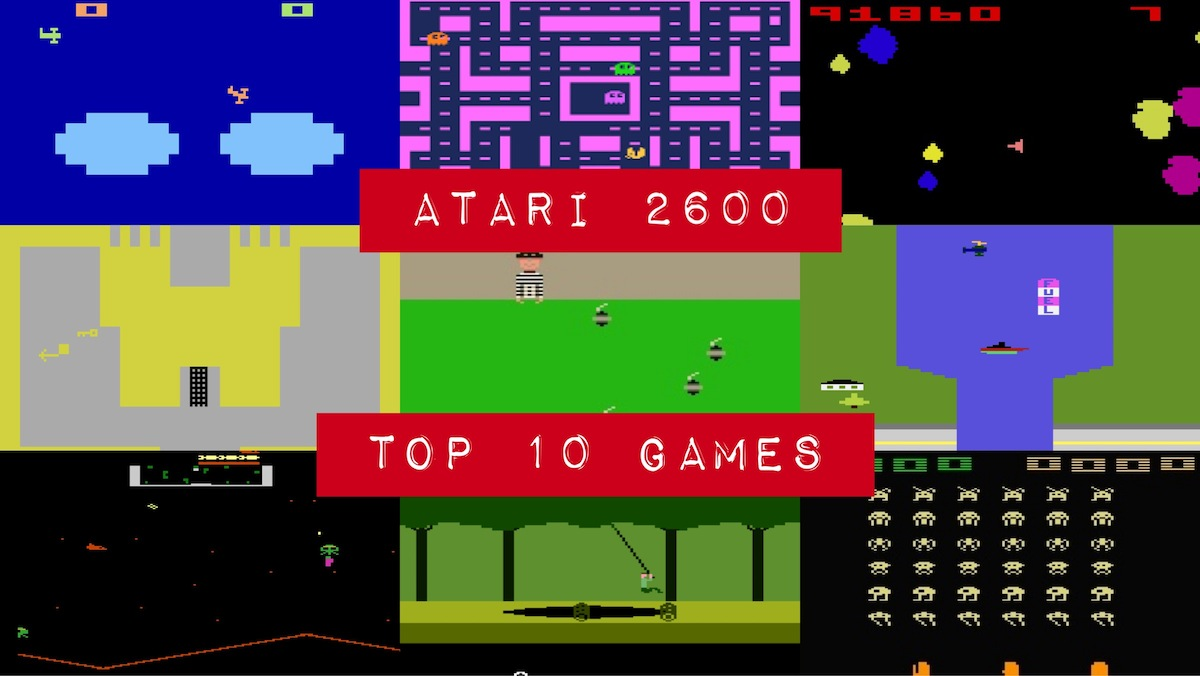
\includegraphics[width=\linewidth]{images/Atari.png}
        \\ \vspace{0.2cm}
        {\small DQN 玩 Atari 游戏}
    \end{column}
    \begin{column}{0.48\textwidth}
        \centering
        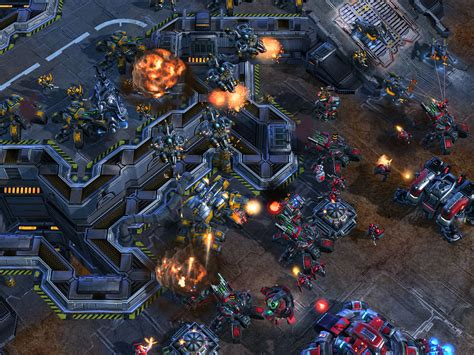
\includegraphics[width=\linewidth]{images/OIP.jpg}
        \\ \vspace{0.2cm}
        {\small 星际争霸}
    \end{column}
\end{columns}
\end{frame}

\begin{frame}{RL在大语言模型中的应用}
  \begin{center}
  \begin{tikzpicture}
      % 每个 node 独立定位，大小可随意调整
      \node at (0,0) {
\includegraphics[width=2cm]{images/chatgpt.jpg}};
      \node at (2.5,0.5) {
\includegraphics[width=3cm]{images/deepseek_icon.jpg}};
      \node at (1,-2) {
\includegraphics[width=2.5cm]{images/cursor_icon.jpg}};
      \node at (5,-2) {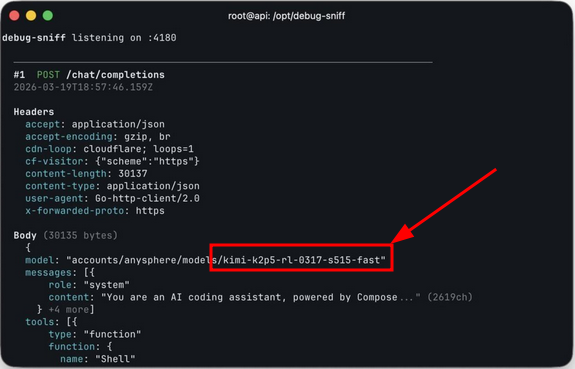
\includegraphics[width=5cm]{images/cursor_kimi.png}};
  \end{tikzpicture}
  \end{center}
{\scriptsize 参考：\cite{research2026composer2technicalreport}}\\
{\scriptsize 参考：\href{https://www.bilibili.com/video/BV1darmBcE4A/?share_source=copy_web&vd_source=ac36b9d866cfcdf1b2e7d9066e87242c}{翁家翌：OpenAI，GPT，强化学习, WhynotTV Podcast #4}}

\end{frame}

% 仅仅是一种RL算法，并不是比PPO更优
% Deepseek GRPO
\begin{frame}{Reinforcement Learning for Human Feedback (RLHF)}
{\scriptsize post-training(后训练)}
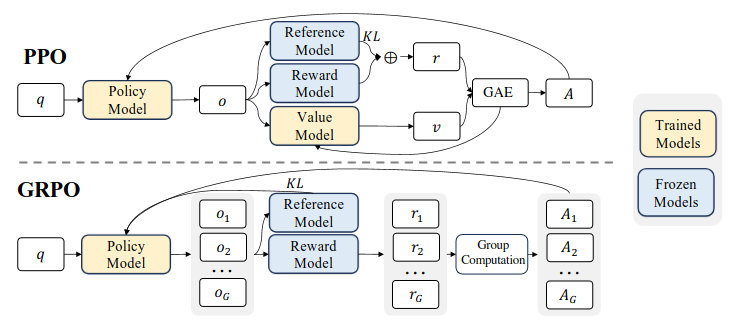
\includegraphics[width=\linewidth]{images/GRPO.png}
{\scriptsize 参考：\cite{shao2024deepseekmathpushinglimitsmathematical}}
\end{frame}


\begin{frame}{机器人运动控制、规划感知}
  \begin{center}
  \begin{minipage}{0.3\textwidth}
          \centering
          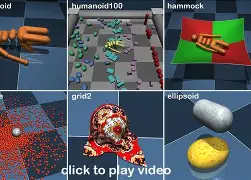
\includegraphics[width=\linewidth]{images/mujoco.png}
          \\[0.1cm]
          {\scriptsize mujoco}
      \end{minipage}
      \hfill  % 自动填充间距
      % 第二张图
      \begin{minipage}{0.3\textwidth}
          \centering
          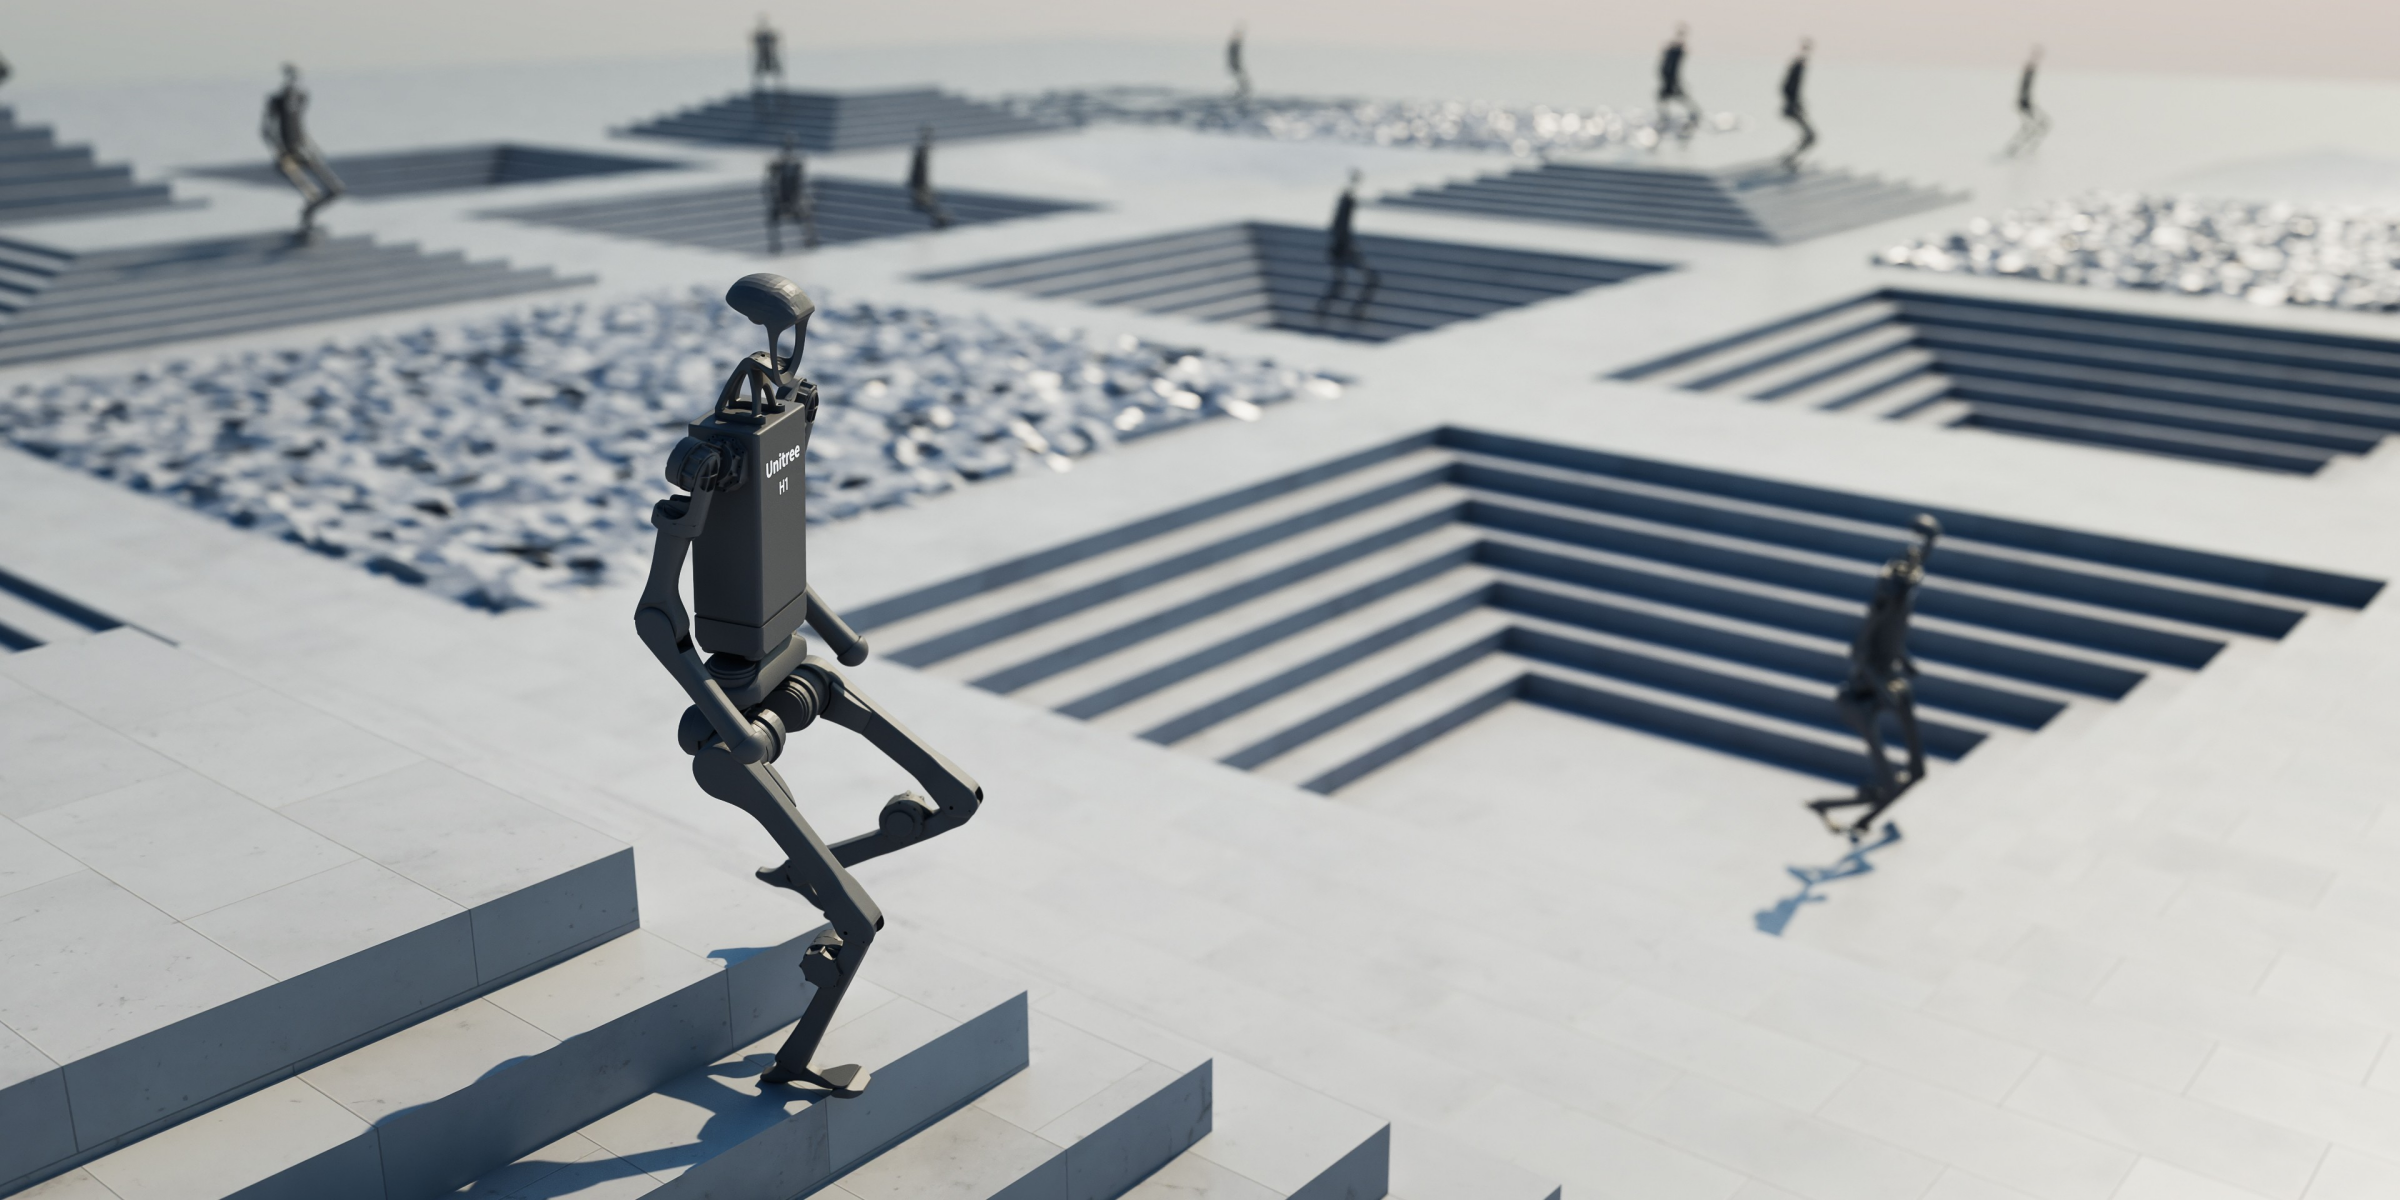
\includegraphics[width=\linewidth]{images/isaacsim.png}
          \\[0.1cm]
          {\scriptsize isaacsim}
      \end{minipage}
      \hfill
      % 第三张图
      \begin{minipage}{0.3\textwidth}
          \centering
          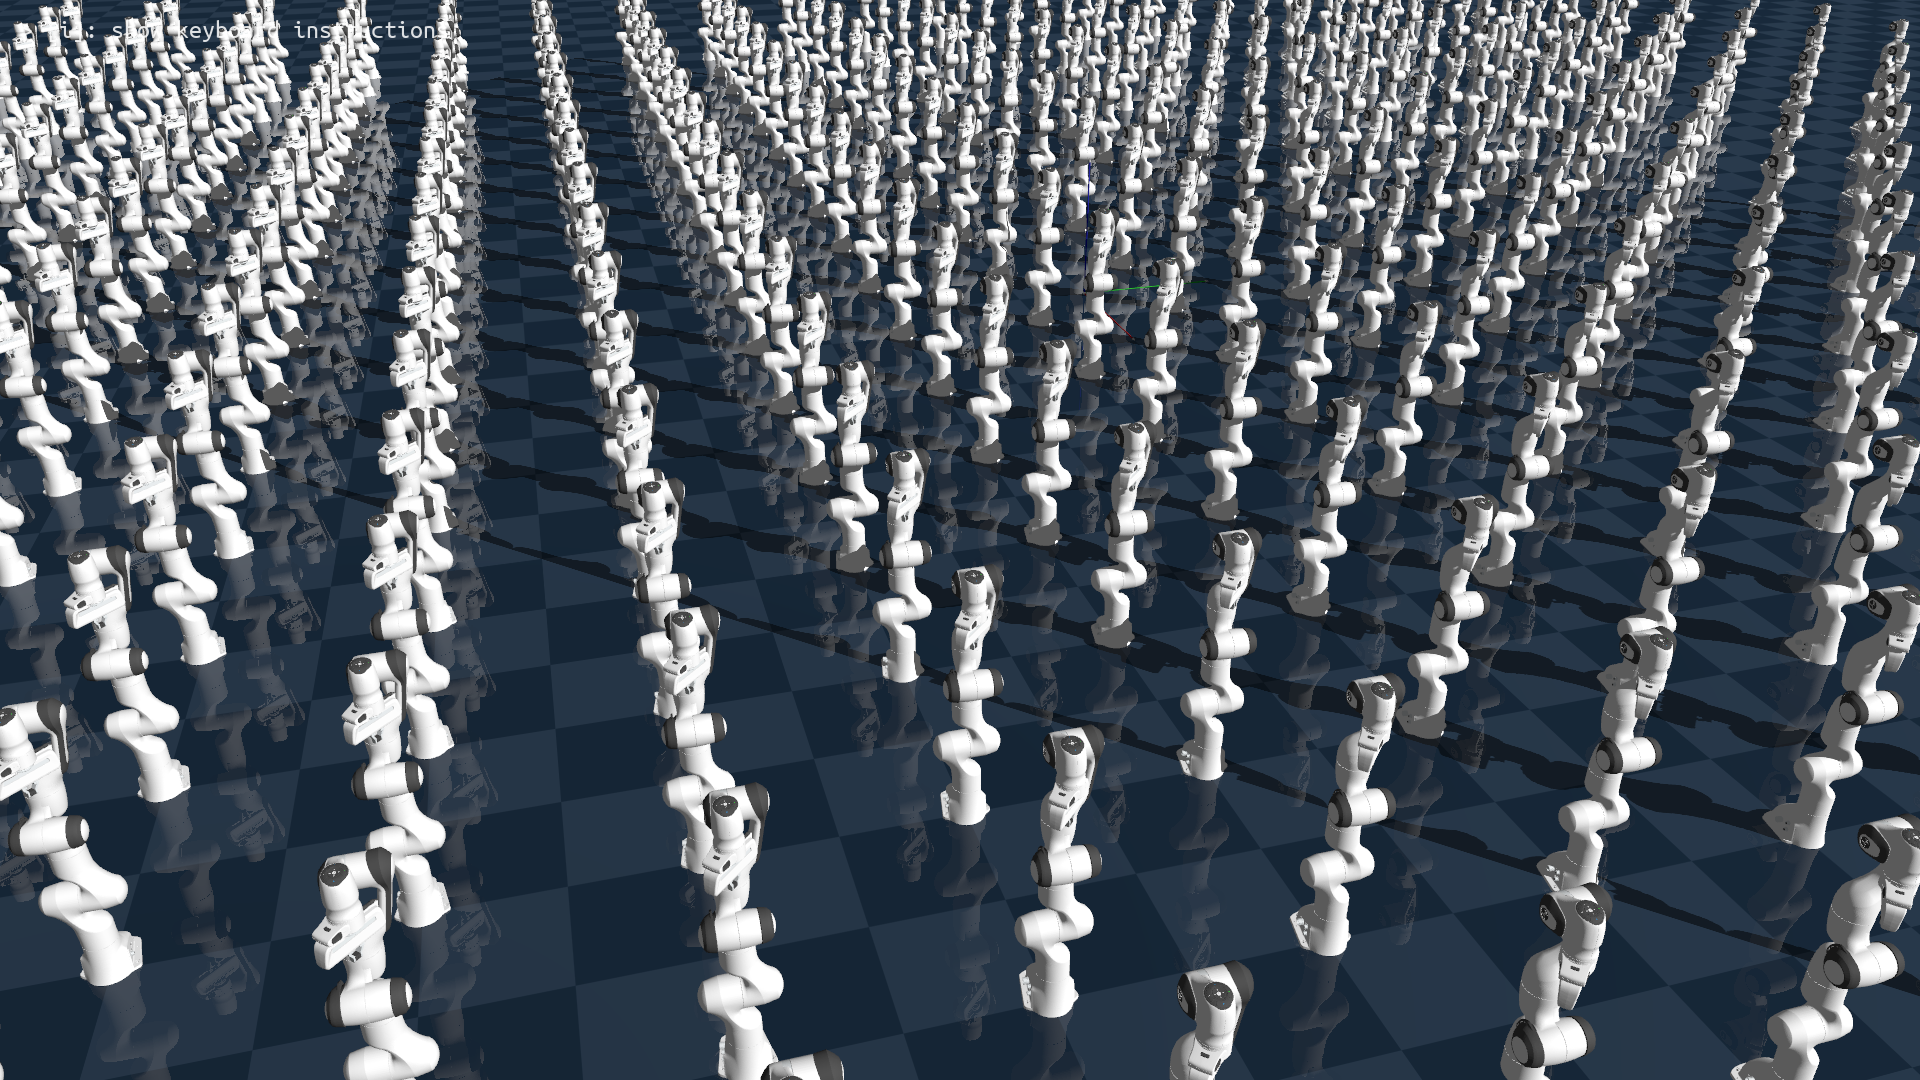
\includegraphics[width=\linewidth]{images/genesis.png}
          \\[0.1cm]
          {\scriptsize genesis}
      \end{minipage}
  \end{center}
{\scriptsize 典型平台：MuJoCo, Isaac Sim, Genesis}

\end{frame}


\section{强化学习几大分类}
\begin{frame}{RL overview}
    \centering
    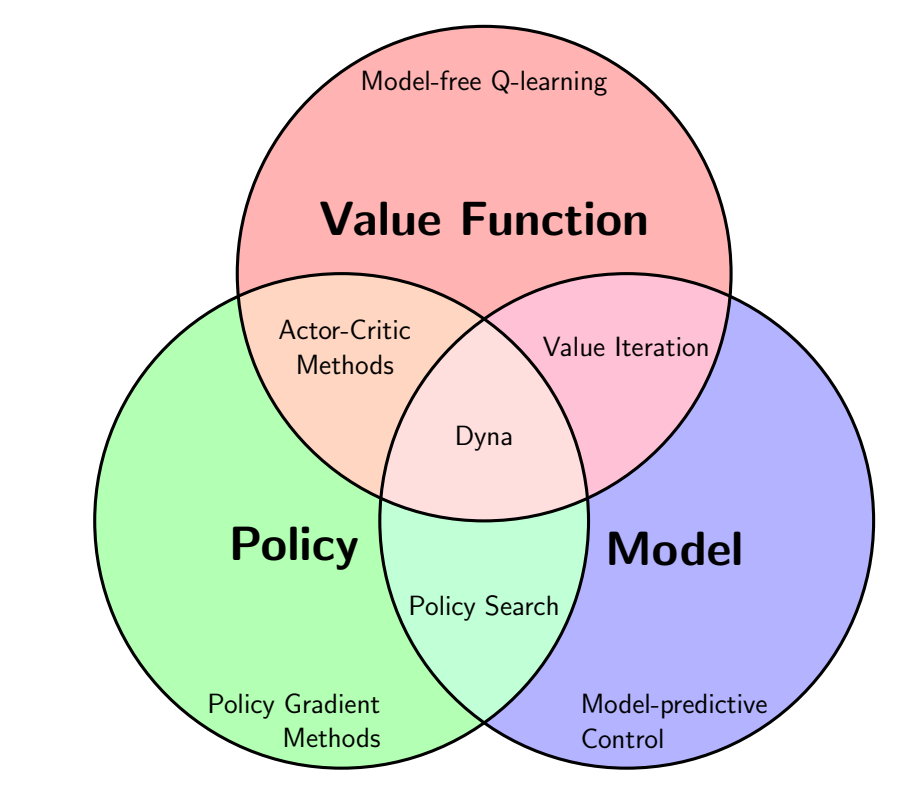
\includegraphics[width=0.7\textwidth]{images/RL_overview.png}
    
    \vspace{0.2cm}
    {\small 从“是否建模环境”“如何表示策略”“数据从哪里来”三个维度理解 RL 算法族谱。}
\end{frame}

\begin{frame}{强化学习的常见分类维度}
\small
\begin{tabular}{p{2.6cm}p{3.1cm}p{4.8cm}}
\toprule
\textbf{分类维度} & \textbf{代表类型} & \textbf{核心区别} \\
\midrule
环境建模 & Model-Free / Model-Based & 是否显式学习环境动力学 $P(s'|s,a)$ 或奖励模型 \\
策略更新 & Value-Based / Policy-Based / Actor-Critic & 通过值函数选动作、直接优化策略、或两者结合 \\
数据来源 & Online / Offline & 数据来自实时交互，还是历史数据集 \\
采样方式 & On-Policy / Off-Policy & 更新时是否只能使用当前策略收集的数据 \\
动作空间 & Discrete / Continuous & 动作是有限集合，还是连续向量控制量 \\
\bottomrule
\end{tabular}

\vspace{0.2cm}
{\scriptsize DQN 常用于离散动作；PPO 常用于稳定的 on-policy 更新；SAC 常用于连续控制与高样本效率场景。}
\end{frame}

\subsection{model-free RL}

\begin{frame}{model-free RL}
    \centering
    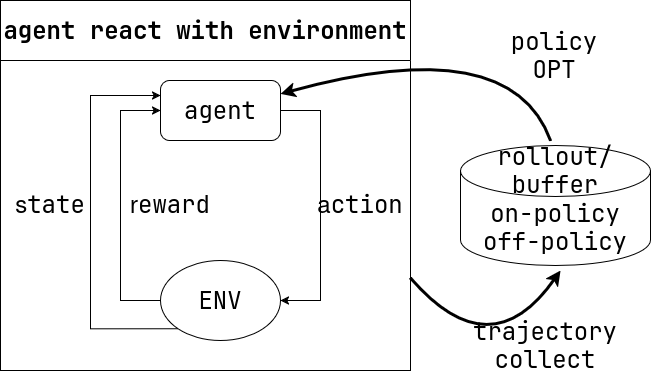
\includegraphics[height=0.5\textwidth]{images/model-free_RL.png}
    
    
\end{frame}

\subsection{model-based RL}

\begin{frame}{model-based RL}
    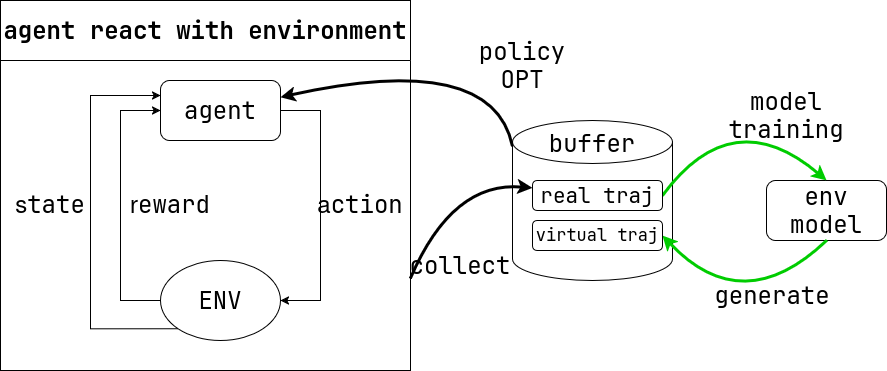
\includegraphics[width=0.9\textwidth]{images/model-based_RL.png}

\end{frame}

\subsection{offline RL(离线强化学习)}

\begin{frame}{offline RL}
\begin{block}{定义}
    离线强化学习（Offline RL）只使用预先收集好的历史数据集训练策略，不再与环境持续交互。
\end{block}

\textbf{典型来源：}
\begin{itemize}
    \item 人类专家示范数据
    \item 旧版本策略产生的日志
    \item 仿真器离线生成的大规模轨迹
\end{itemize}

\textbf{难点：}
\begin{itemize}
    \item 分布外动作（OOD action）会导致 Q 值高估
    \item 无法通过重新试错修正错误估计
\end{itemize}
\end{frame}

\subsection{online RL(在线强化学习)}

\begin{frame}{online RL}
\begin{block}{定义}
    在线强化学习（Online RL）在训练过程中持续与环境交互，边采样边更新。
\end{block}

\textbf{优势：}
\begin{itemize}
    \item 数据与当前策略匹配，反馈闭环清晰
    \item 可以通过探索不断改善策略
\end{itemize}

\textbf{代价：}
\begin{itemize}
    \item 需要大量环境交互，样本成本高
    \item 在真实机器人、医疗、金融等场景试错代价很高
\end{itemize}
\end{frame}

\section{值函数方法}

\begin{frame}{值函数方法：背景与动机}
    \begin{block}{核心思想}
        值函数方法通过学习\textbf{状态值函数} $V(s)$ 或 \textbf{动作值函数} $Q(s,a)$ 来评估策略的好坏，从而间接地优化策略。
    \end{block}
    
    \vspace{0.3cm}
    
    \textbf{值函数的定义：}
    \begin{itemize}
        \item \textbf{状态值函数}：从状态 $s$ 开始，遵循策略 $\pi$ 的期望累积奖励
        \[ V^\pi(s) = \mathbb{E}_\pi \left[ \sum_{t=0}^{\infty} \gamma^t r_t \Big| s_0 = s \right] \]
        \item \textbf{动作值函数}：在状态 $s$ 执行动作 $a$ 后，遵循策略 $\pi$ 的期望累积奖励
        \[ Q^\pi(s,a) = \mathbb{E}_\pi \left[ \sum_{t=0}^{\infty} \gamma^t r_t \Big| s_0 = s, a_0 = a \right] \]
    \end{itemize}
    
    \vspace{0.2cm}
    {\small 关系：$V^\pi(s) = \sum_a \pi(a|s) Q^\pi(s,a)$}
\end{frame}

\begin{frame}{Bellman方程与最优性}
    \begin{block}{Bellman期望方程}
        值函数满足自洽性方程：
        \begin{align*}
        V^\pi(s) &= \sum_a \pi(a|s) \sum_{s'} P(s'|s,a) \left[ R(s,a,s') + \gamma V^\pi(s') \right] \\
        Q^\pi(s,a) &= \sum_{s'} P(s'|s,a) \left[ R(s,a,s') + \gamma \sum_{a'} \pi(a'|s') Q^\pi(s',a') \right]
        \end{align*}
    \end{block}
\end{frame}

\begin{frame}{Bellman最优方程}
    \begin{block}{Bellman最优方程}
        最优值函数满足：
        \begin{align*}
        V^*(s) &= \max_a \sum_{s'} P(s'|s,a) \left[ R(s,a,s') + \gamma V^*(s') \right] \\
        Q^*(s,a) &= \sum_{s'} P(s'|s,a) \left[ R(s,a,s') + \gamma \max_{a'} Q^*(s',a') \right]
        \end{align*}
    \end{block}
    
    \vspace{0.3cm}
    
    \begin{block}{最优策略}
        \[
        \pi^*(a|s) = \arg\max_a Q^*(s,a)
        \]
        选择使Q值最大的动作
    \end{block}
\end{frame}

\begin{frame}{值函数估计方法}
    \textbf{1. 蒙特卡洛方法（MC）：}
    \begin{itemize}
        \item 通过完整采样轨迹估计值函数
        \item $V(s) \approx \frac{1}{N} \sum_{i=1}^N G_i$，其中 $G_i$ 是第 $i$ 次访问 $s$ 的累计回报
    \end{itemize}
    
    \vspace{0.3cm}
    
    \textbf{2. 时序差分学习（TD）：}
    \begin{itemize}
        \item 用当前估计更新值函数，无需等待轨迹结束
        \item \textbf{TD(0)}：$V(s_t) \leftarrow V(s_t) + \alpha [r_t + \gamma V(s_{t+1}) - V(s_t)]$
        \item \textbf{SARSA}（同策略）：
        \[ Q(s_t,a_t) \leftarrow Q(s_t,a_t) + \alpha [r_t + \gamma Q(s_{t+1},a_{t+1}) - Q(s_t,a_t)] \]
        \item \textbf{Q-Learning}（异策略）：
        \[ Q(s_t,a_t) \leftarrow Q(s_t,a_t) + \alpha [r_t + \gamma \max_a Q(s_{t+1},a) - Q(s_t,a_t)] \]
    \end{itemize}
\end{frame}

\subsection{DQN}

\begin{frame}{Deep Q-Network (DQN)}
    \begin{columns}[T]
        \begin{column}{0.65\textwidth}
            \begin{block}{背景}
                \begin{itemize}
                    \item \textbf{2015年}，DeepMind发表在\textit{Nature}
                    \item 首次成功将深度学习与强化学习结合
                    \item 在Atari 2600游戏上达到人类水平
                \end{itemize}
            \end{block}
            
            \textbf{核心问题：}\\
            传统Q-Learning在高维连续状态空间（如图像）无法存储$Q$表
            
            \textbf{解决方案：}\\
            使用深度神经网络近似Q函数：
            \[ Q(s,a;\theta) \approx Q^*(s,a) \]
        \end{column}
        
        \begin{column}{0.4\textwidth}
            \centering
            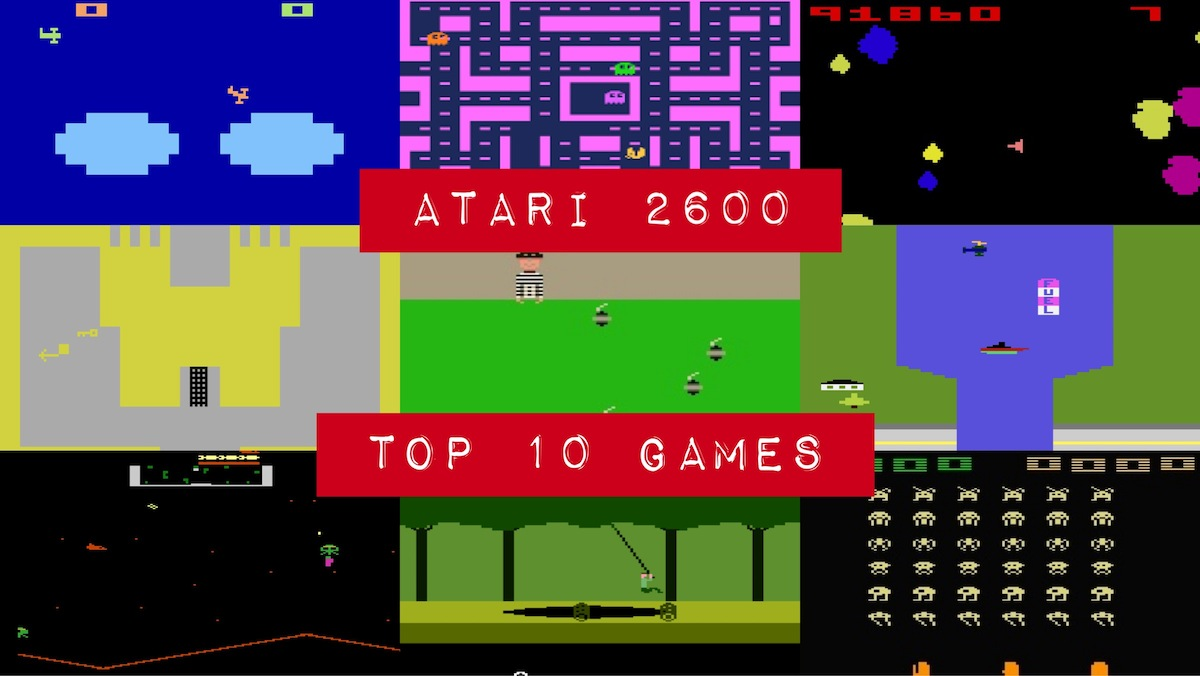
\includegraphics[width=\textwidth]{images/Atari.png}\\
            {\scriptsize DQN在Atari上的表现}
        \end{column}
    \end{columns}
\end{frame}

\begin{frame}{DQN：损失函数与目标网络}
    \begin{block}{DQN损失函数}
        最小化当前Q值与目标Q值的均方误差：
        \[ L(\theta) = \mathbb{E}_{(s,a,r,s') \sim D} \left[ \left( y - Q(s,a;\theta) \right)^2 \right] \]
        其中目标值为：
        \[ y = r + \gamma \max_{a'} Q(s',a';\theta^-) \]
    \end{block}
    
    \textbf{关键技术1：目标网络（Target Network）}
    \begin{itemize}
        \item 使用独立的参数$\theta^-$计算目标值
        \item 定期从主网络复制：$\theta^- \leftarrow \theta$（每隔$C$步）
        \item 避免自举（bootstrapping）导致的训练不稳定
    \end{itemize}
    
    \textbf{关键技术2：经验回放（Experience Replay）}
    \begin{itemize}
        \item 存储转移样本 $(s, a, r, s')$ 到回放缓冲区$D$
        \item 随机采样打破数据相关性，提高样本效率
    \end{itemize}
\end{frame}

\begin{frame}{DQN算法流程}
    \begin{algorithm}[H]
    \scriptsize
    \caption{DQN算法}
    \begin{algorithmic}[1]
    \STATE 初始化：回放缓冲区$D$，Q网络参数$\theta$，目标网络参数$\theta^- = \theta$
    \FOR{episode = 1, 2, ...}
        \STATE 获得初始状态$s_1$ 
        \FOR{$t = 1, 2, ...$} 
            \STATE 以$\epsilon$-greedy策略选择动作：$a_t \sim \pi_\epsilon(s_t)$ 
            \STATE 执行动作$a_t$，观察奖励$r_t$和下一状态$s_{t+1}$ 
            \STATE 存储转移样本$(s_t, a_t, r_t, s_{t+1})$到回放缓冲区$D$ 
            \STATE 从$D$中随机采样小批量样本$\{(s_j, a_j, r_j, s_{j+1})\}$ 
            \STATE 计算目标值：$y_j = r_j + \gamma \max_{a'} Q(s_{j+1}, a'; \theta^-)$ 
            \STATE 执行梯度下降：$\theta \leftarrow \theta - \alpha \nabla_\theta \sum_j (y_j - Q(s_j, a_j; \theta))^2$ 
            \STATE 每$C$步更新目标网络：$\theta^- \leftarrow \theta$ 
        \ENDFOR 
    \ENDFOR 
    \end{algorithmic} 
    \end{algorithm} 
\end{frame}

\begin{frame}{Double DQN：缓解过估计问题}
    \begin{block}{DQN 的问题}
        在标准 DQN 中，目标值里的 $\max_{a'} Q(s',a';\theta^-)$ 同时承担了\textbf{动作选择}和\textbf{动作评估}两项职责，这会带来系统性的过估计偏差。
    \end{block}

    \textbf{标准 DQN 目标：}
    \[
    y^{DQN} = r + \gamma \max_{a'} Q(s', a'; \theta^-)
    \]

    \textbf{Double DQN 思想：}
    \begin{itemize}
        \item 在线网络 $\theta$ 负责选动作：$a^* = \arg\max_{a'} Q(s',a';\theta)$
        \item 目标网络 $\theta^-$ 负责评估该动作价值
    \end{itemize}

    \textbf{Double DQN 目标：}
    \[
    y^{DDQN} = r + \gamma Q(s', \arg\max_{a'} Q(s',a';\theta); \theta^-)
    \]
\end{frame}

\begin{frame}{Double DQN：为什么更稳定？}
    \begin{columns}[T]
        \begin{column}{0.48\textwidth}
            \begin{block}{核心收益}
                \begin{itemize}
                    \item 将“选最大值”和“评估最大值”分离
                    \item 减少噪声导致的过乐观估计
                    \item 训练更稳定，尤其在 Atari 等离散任务中更明显
                \end{itemize}
            \end{block}
        \end{column}
        \begin{column}{0.48\textwidth}
            \begin{block}{一句话理解}
                标准 DQN 容易“自己挑自己喜欢的动作，再自己夸自己”，Double DQN 用两个网络把这两个动作分开处理。
            \end{block}
            \vspace{0.15cm}
            {\small Double DQN 本质上没有改变 DQN 的整体框架，只是改了 target 的构造方式。}
        \end{column}
    \end{columns}
\end{frame}

\begin{frame}{Dueling DQN：分离状态价值与动作优势}
    \begin{block}{动机}
        在很多状态下，不同动作的价值差别并不大。此时直接学习每个动作的 $Q(s,a)$ 往往低效。
    \end{block}

    \textbf{Dueling Network 结构：}
    \begin{itemize}
        \item Value stream：学习状态价值 $V(s)$
        \item Advantage stream：学习动作优势 $A(s,a)$
        \item 最后组合为动作价值 $Q(s,a)$
    \end{itemize}

    \[
    Q(s,a) = V(s) + \left( A(s,a) - \frac{1}{|\mathcal{A}|}\sum_{a'} A(s,a') \right)
    \]

    {\small 减去平均优势项是为了让分解更稳定，避免 $V$ 和 $A$ 的表示不唯一。}
\end{frame}

\begin{frame}{Dueling DQN：适合什么场景？}
    \begin{columns}[T]
        \begin{column}{0.48\textwidth}
            \textbf{适合的状态：}
            \begin{itemize}
                \item 很多动作都差不多时
                \item 更关心“当前状态值不值得”而不是“每个动作差异有多大”
                \item 动作空间较大、冗余动作较多的离散控制任务
            \end{itemize}
        \end{column}
        \begin{column}{0.48\textwidth}
            \textbf{实践效果：}
            \begin{itemize}
                \item 更快识别“好状态 / 坏状态”
                \item 在不显著增加采样成本的情况下提升性能
                \item 常与 Double DQN、Prioritized Replay 一起组合
            \end{itemize}
        \end{column}
    \end{columns}
    \vspace{0.2cm}
    \begin{block}{总结}
        Double DQN 改的是\textbf{目标值估计偏差}，Dueling DQN 改的是\textbf{网络表示能力}。
    \end{block}
\end{frame}
\begin{frame}{Bootstrapping}

\includegraphics[width=\linewidth]{images/dog_eat_tail.jpg}

\vspace{0.15cm}
{\small 自举（bootstrapping）指用当前估计值去更新未来估计值。它提高了样本效率，但也可能带来偏差与不稳定。}
\end{frame}
\section{策略梯度方法}

\begin{frame}{策略梯度方法：背景与动机}
    \begin{block}{核心思想}
        直接对策略$\pi_\theta(a|s)$进行参数化，通过梯度上升优化策略参数$\theta$，使期望累积奖励最大化。
    \end{block}
    
    \textbf{目标函数：}
    \[ J(\theta) = \mathbb{E}_{\tau \sim \pi_\theta} \left[ \sum_{t=0}^{T} r(s_t, a_t) \right] \]
    
    \begin{block}{策略梯度定理}
        \[ \nabla_\theta J(\theta) = \mathbb{E}_{\pi_\theta} \left[ \nabla_\theta \log \pi_\theta(a|s) \cdot Q^{\pi_\theta}(s,a) \right] \]
    \end{block}
    {\scriptsize 直观解释：增加高回报状态-动作对的对数概率，降低低回报的对数概率}
\end{frame}

\begin{frame}{策略梯度定理推导}
    \textbf{步骤1：将目标函数展开}
    \begin{align*}
    J(\theta) &= \mathbb{E}_{\tau \sim \pi_\theta} [R(\tau)] = \int P(\tau|\theta) R(\tau) d\tau \\
    \nabla_\theta J(\theta) &= \int \nabla_\theta P(\tau|\theta) R(\tau) d\tau
    \end{align*}
    
    \textbf{步骤2：利用对数导数技巧}
    \[ \nabla_\theta P(\tau|\theta) = P(\tau|\theta) \nabla_\theta \log P(\tau|\theta) \]
    \vspace{-0.2cm}
    \textbf{步骤3：轨迹概率分解}
    \vspace{-0.4cm}
    \[P(\tau|\theta) = P(s_0) \prod_{t=0}^{T} \pi_\theta(a_t|s_t) P(s_{t+1}|s_t, a_t) \]
    \vspace{-0.2cm}
    \textbf{步骤4：求梯度}
    \vspace{-0.2cm}
     \[ \nabla_\theta \log P(\tau|\theta) = \sum_{t=0}^{T} \nabla_\theta \log \pi_\theta(a_t|s_t) \]{\small \textbf{注：}更详细的推导涉及到信息几何，这里只是简单的推导}
    
\end{frame}

\begin{frame}{对数导数技巧}

        对于概率分布 $P(x|\theta)$，我们希望计算 $\nabla_\theta P(x|\theta)$
    
    \textbf{步骤1：取对数}
    \[
    \log P(x|\theta)
    \]
    
    \textbf{步骤2：对对数求导（链式法则）}
    \[
    \nabla_\theta \log P(x|\theta) = \frac{1}{P(x|\theta)} \cdot \nabla_\theta P(x|\theta)
    \]
    
    \textbf{步骤3：}
        \[
        \nabla_\theta P(x|\theta) = P(x|\theta) \cdot \nabla_\theta \log P(x|\theta)
        \]
\end{frame}

\begin{frame}{为什么使用对数导数？}
    \textbf{场景：轨迹概率是乘积形式}
    \[
    P(\tau|\theta) = P(s_0) \prod_{t=0}^{T} \pi_\theta(a_t|s_t) P(s_{t+1}|s_t, a_t)
    \]
    
    \textbf{直接求导的问题：}
    \begin{itemize}
        \item 需要使用乘积法则，产生 $2^T$ 项
        \item 计算复杂度随轨迹长度指数增长
        \item 实现困难，容易出错
    \end{itemize}
    
    \textbf{取对数后的优势：}
    \[
    \log P(\tau|\theta) = \log P(s_0) + \sum_{t=0}^{T} \left[ \log \pi_\theta(a_t|s_t) + \log P(s_{t+1}|s_t, a_t) \right]
    \]
    
    \begin{itemize}
        \item \textbf{乘法变加法}：求导简单
        \item \textbf{环境项消失}：$P(s_{t+1}|s_t, a_t)$ 不依赖 $\theta$
    \end{itemize}
\end{frame}

\begin{frame}{轨迹概率求导的具体过程}
    \textbf{轨迹概率的对数：}
    \[
    \log P(\tau|\theta) = \underbrace{\log P(s_0)}_{\text{初始状态}} + \sum_{t=0}^{T} \underbrace{\log \pi_\theta(a_t|s_t)}_{\text{策略}} + \sum_{t=0}^{T} \underbrace{\log P(s_{t+1}|s_t, a_t)}_{\text{环境转移}}
    \]
    
    \textbf{对 $\theta$ 求导：}
    \[
    \nabla_\theta \log P(\tau|\theta) = \nabla_\theta \log P(s_0) + \sum_{t=0}^{T} \nabla_\theta \log \pi_\theta(a_t|s_t) + \sum_{t=0}^{T} \nabla_\theta \log P(s_{t+1}|s_t, a_t)
    \]
    
    \textbf{简化（只有策略依赖 $\theta$）：}
        \[
        \nabla_\theta \log P(\tau|\theta) = \sum_{t=0}^{T} \nabla_\theta \log \pi_\theta(a_t|s_t)
        \]
    
    {\small 关键洞察：环境转移概率 $P(s'|s,a)$ 与策略参数 $\theta$ 无关！}
\end{frame}

\begin{frame}{REINFORCE算法}
    \begin{block}{蒙特卡洛策略梯度}
        使用实际回报$G_t$估计$Q^{\pi}(s,a)$：
        \[ \nabla_\theta J(\theta) = \mathbb{E}_{\pi_\theta} \left[ \sum_{t=0}^{T} \nabla_\theta \log \pi_\theta(a_t|s_t) \cdot G_t \right] \]
        其中$G_t = \sum_{k=t}^{T} \gamma^{k-t} r_k$是从时间步$t$开始的折扣回报。
    \end{block}
    
    \textbf{REINFORCE算法流程：}
    \begin{itemize}
        \item 根据$\pi_\theta$采样完整轨迹$\tau$
        \item 对每个时间步$t$：
        \item 计算累计回报：$G_t = \sum_{k=t}^{T} \gamma^{k-t} r_k$
        \item 更新参数：$\theta \leftarrow \theta + \alpha \nabla_\theta \log \pi_\theta(a_t|s_t) G_t$
    \end{itemize}
    
    {\small \textbf{问题}：高方差，需要完整轨迹}
\end{frame}
% reinforce with baseline
\begin{frame}{REINFORCE with baseline}
          可以在策略梯度中加入任意与动作无关的 baseline $b(s)$：
          \[
          \nabla_\theta J(\theta)
          \propto
          \sum_s \mu(s)\sum_a \bigl(q_\pi(s,a)-b(s)\bigr)\nabla_\theta \pi_\theta(a|s)
          \]
          \[
          =
          \sum_s \mu(s)\left[
          \sum_a q_\pi(s,a)\nabla_\theta \pi_\theta(a|s)
          -
          b(s)\nabla_\theta \sum_a \pi_\theta(a|s)
          \right]
          \]
          \[
          =
          \sum_s \mu(s)\sum_a q_\pi(s,a)\nabla_\theta \pi_\theta(a|s),
          \qquad
          \text{因为 } \nabla_\theta\sum_a \pi_\theta(a|s)=1.
          \]
      {\small 常用选择是 $b(s_t)=V^\pi(s_t)$，此时 $G_t-b(s_t)$ 可看作 advantage 的估计}
  \end{frame}

\begin{frame}{Actor-Critic架构}

            \begin{block}{核心思想}
                结合\textbf{策略梯度}（Actor）和\textbf{值函数估计}（Critic）：
                \begin{itemize}
                    \item \textbf{Actor}：策略网络$\pi_\theta(a|s)$，负责选择动作
                    \item \textbf{Critic}：值函数网络$V_\phi(s)$，评估动作好坏
                \end{itemize}
            \end{block}
            
            \textbf{优势函数：}
            \[ A(s,a) = Q(s,a) - V(s) \]
 \vspace{0.3cm}
    \centering
    \begin{tikzpicture}[scale=0.7]
        \node[draw, rounded corners, fill=blue!20, minimum width=2cm, minimum height=1cm] (env) at (0,0) {环境};
        \node[draw, rounded corners, fill=red!20, minimum width=2cm, minimum height=1cm] (actor) at (-3,2) {Actor};
        \node[draw, rounded corners, fill=green!20, minimum width=2cm, minimum height=1cm] (critic) at (3,2) {Critic};
        
        \draw[->, thick] (env) -- (actor) node[midway, left] {$s_t$};
        \draw[->, thick] (actor) -- (env) node[midway, left] {$a_t$};
        \draw[->, thick] (env) -- (critic) node[midway, right] {$r_t, s_{t+1}$};
        \draw[->, thick, dashed] (critic) -- (actor) node[midway, above] {$A(s,a)$};
    \end{tikzpicture}
\end{frame}

\subsection{PPO}
\begin{frame}{Proximal Policy Optimization (PPO)}
    \begin{block}{简介}
        \begin{itemize}
            \item \textbf{2017年}，OpenAI提出（Schulman et al.）
            \item 解决策略梯度方法中的\textbf{更新步长敏感}问题
            \item 避免策略更新过大导致性能崩溃
        \end{itemize}
    \end{block}
    
    \vspace{0.3cm}
    
    \textbf{重要性采样比率：}
    \[ r_t(\theta) = \frac{\pi_\theta(a_t|s_t)}{\pi_{\theta_{old}}(a_t|s_t)} \]
    
    \vspace{0.3cm}
    
    \textbf{PPO-Clip目标函数：}
    \[ L^{CLIP}(\theta) = \mathbb{E} \left[ \min\left( r_t(\theta) A_t, \text{clip}(r_t(\theta), 1-\epsilon, 1+\epsilon) A_t \right) \right] \]
    
    \cite{schulman2017proximalpolicyoptimizationalgorithms}
\end{frame}

\begin{frame}{PPO：目标函数与裁剪机制}
    \begin{columns}[T]
        \begin{column}{0.5\textwidth}
            \textbf{完整目标函数：}
            \[ L^{TOTAL}(\theta) = \mathbb{E} \left[ L^{CLIP}(\theta) - c_1 (V_\phi(s) - V_t^{target})^2 + c_2 \mathcal{H}(\pi_\theta(\cdot|s)) \right] \]
            
            \vspace{0.3cm}

                \begin{itemize}
                    \item $L^{CLIP}$：策略Clip损失
                    \item $c_1 (V_\phi - V^{target})^2$：值函数损失
                    \item $c_2 \mathcal{H}(\pi_\theta)$：熵奖励（探索）
                \end{itemize}
        \end{column}
        
        \begin{column}{0.45\textwidth}
    \vspace*{1.5cm}
\begin{block}{裁剪机制}\\
         $r_t(\theta) \in [1-\epsilon, 1+\epsilon]$\\
    \textbf{当 $A_t > 0$（好动作）：}
     \item 若 $r_t > 1+\epsilon$：停止增加概率,防止过度优化\\
    \textbf{当 $A_t < 0$（坏动作）：}
    \item 若 $r_t < 1-\epsilon$：停止减小概率,防止过度惩罚
\end{block}
\end{column}
\end{columns}
\end{frame}

\begin{frame}{重要性采样（Importance Sampling）}

        \begin{itemize}
            \item 策略梯度是\textbf{同策略（on-policy）}方法：只能用当前策略收集的数据
            \item 数据效率低：每次更新后，旧数据就不能用了
            \item 重要性采样允许用\textbf{旧策略}的数据更新\textbf{新策略}
        \end{itemize}

    \textbf{重要性采样比率}：
        \[
        r_t(\theta) = \frac{\pi_\theta(a_t|s_t)}{\pi_{\theta_{old}}(a_t|s_t)}
        \]

    \begin{itemize}
        \item $r_t(\theta) > 1$：新策略比旧策略更倾向于选择动作$a_t$
        \item $r_t(\theta) < 1$：新策略比旧策略更不倾向于选择动作$a_t$
        \item $r_t(\theta) = 1$：新旧策略对该动作的偏好相同
    \end{itemize}
\end{frame}

\begin{frame}{Generalized Advantage Estimation (GAE)}
    \begin{block}{背景与动机}
        \begin{itemize}
            \item 策略梯度需要准确估计优势函数 $A(s,a) = Q(s,a) - V(s)$
            \item MC方法方差大，TD方法有偏
            \item GAE在偏差和方差之间进行权衡
        \end{itemize}
    \end{block}
    
    \textbf{TD残差（单步）}：
    \[
    \delta_t = r_t + \gamma V(s_{t+1}) - V(s_t)
    \]
    
    \textbf{GAE($\lambda$)定义}：
    \[
    \hat{A}_t^{GAE(\lambda)} = \sum_{l=0}^{\infty} (\gamma\lambda)^l \delta_{t+l}
    \]
    
    展开形式：
    \[
    \hat{A}_t = \delta_t + (\gamma\lambda)\delta_{t+1} + (\gamma\lambda)^2\delta_{t+2} + \cdots
    \]
\end{frame}

\begin{frame}{GAE：参数解释与计算}
    \textbf{参数 $\lambda$ 的作用：}
    \begin{itemize}
        \item $\lambda = 0$：退化为单步TD，$\hat{A}_t = \delta_t$（偏差大，方差小）
        \item $\lambda = 1$：退化为MC，$\hat{A}_t = \sum_{l=0}^{\infty}\gamma^l r_{t+l} - V(s_t)$（偏差小，方差大）
        \item $0 < \lambda < 1$：偏差和方差的折中
    \end{itemize}
    
    \vspace{0.3cm}
    
    \textbf{实际计算（截断版本）}：
    \begin{align*}
    \hat{A}_t &= \delta_t + (\gamma\lambda)\delta_{t+1} + (\gamma\lambda)^2\delta_{t+2} + \cdots + (\gamma\lambda)^{T-t-1}\delta_{T-1}
    \end{align*}
    
    \vspace{0.3cm}
    {\small 实际应用中通常取 $\lambda = 0.95$，$\gamma = 0.99$}
\end{frame}

\begin{frame}{PPO算法流程：采样与优势估计}
    \begin{enumerate}
        \item 初始化策略网络 $\pi_\theta$ 与值函数网络 $V_\phi$
        \item 用当前旧策略 $\pi_{\theta_{old}}$ 与环境交互，收集一批轨迹数据
        \item 对每个时间步计算 TD 残差：
        \[
        \delta_t = r_t + \gamma V_\phi(s_{t+1}) - V_\phi(s_t)
        \]
        \item 用 GAE 计算优势，再构造回报：
        \[
        \hat{A}_t = \sum_{l=0}^{T-t-1}(\gamma \lambda)^l \delta_{t+l}, \qquad
        G_t = \hat{A}_t + V_\phi(s_t)
        \]
    \end{enumerate}

    \vspace{0.2cm}
    {\small 这一阶段的目标是把原始轨迹转成适合优化的训练信号：优势 $\hat{A}_t$ 和回报 $G_t$。}
\end{frame}

\begin{frame}{PPO算法流程：小批量更新}
    \begin{enumerate}
        \item 固定旧策略参数 $\theta_{old}$，将轨迹数据打乱为多个 mini-batch
        \item 计算重要性采样比率：
        \[
        r_t(\theta) = \frac{\pi_\theta(a_t|s_t)}{\pi_{\theta_{old}}(a_t|s_t)}
        \]
        \item 计算裁剪目标并更新策略：
        \[
        L^{CLIP} = \min\left( r_t(\theta) A_t,\ \text{clip}(r_t(\theta),1-\epsilon,1+\epsilon)A_t \right)
        \]
        \item 同时最小化值函数误差，重复 $K$ 个 epoch 后令 $\theta_{old} \leftarrow \theta$
    \end{enumerate}

    \begin{block}{直观理解}
        PPO 的本质是“\textbf{用旧数据多次更新，但不允许新策略一步走太远}”。
    \end{block}
\end{frame}
\begin{frame}{PPO}
    \begin{block}{连续动作空间下如何计算重要性采样？}
    \end{block}
        $$r_t(\theta) = \frac{\pi_\theta(a_t|s_t)}{\pi_{\theta_{old}}(a_t|s_t)} = \frac{p_\theta(a_t|s_t)}{p_{\theta_{old}}(a_t|s_t)}$$
连续动作通常用高斯分布：
$$\pi_\theta(a|s) = \mathcal{N}(\mu_\theta(s), \Sigma_\theta(s))$$

\vspace{0.2cm}
{\small 对连续动作来说，$\pi_\theta(a|s)$ 不是概率质量，而是\textbf{概率密度}，因此实现时通常在对数密度空间中计算比率。}

\end{frame}
\begin{frame}{PPO：连续动作空间计算细节}

计算步骤：\\
1. 计算对数概率密度：
$$\log \pi_\theta(a|s) = -\frac{1}{2}\sum_{i=1}^d \left[\frac{(a_i - \mu_i)^2}{\sigma_i^2} + \log(2\pi\sigma_i^2)\right]$$
2. 重要性采样比率：
$$\log r_t(\theta) = \log \pi_\theta(a_t|s_t) - \log \pi_{\theta_{old}}(a_t|s_t)$$
3. 取指数得到比率：
$$r_t(\theta) = \exp\left(\log r_t(\theta)\right)$$

\vspace{0.2cm}
{\small 实际实现中策略网络通常输出 $\mu_\theta(s)$ 和 $\log \sigma_\theta(s)$，这样更方便约束方差为正，并避免数值下溢。}

\end{frame}
\subsection{SAC}
\begin{frame}{Soft Actor-Critic (SAC)}
    \begin{block}{简介}
        \begin{itemize}
            \item \textbf{2018年}，UC Berkeley提出（Haarnoja et al.）
            \item 基于\textbf{最大熵强化学习}（Maximum Entropy RL）框架
            \item 目标是学习一个\textbf{随机策略}，同时最大化奖励和策略熵
        \end{itemize}
    \end{block}
    
    \textbf{最大熵目标函数：}
    \[ J(\pi) = \mathbb{E}_{\rho_\pi} \left[ \sum_{t=0}^{\infty} \gamma^t \left( r(s_t, a_t) + \alpha \mathcal{H}(\pi(\cdot|s_t)) \right) \right] \]
    
    其中$\mathcal{H}(\pi(\cdot|s)) = -\mathbb{E}_{a \sim \pi} [\log \pi(a|s)]$是策略熵
    
    \textbf{最优策略形式：}
        \[ \pi^*(a|s) \propto \exp\left( \frac{1}{\alpha} Q^{soft}(s,a) \right) \]
\end{frame}

\begin{frame}{SAC：为什么适合连续控制？}
    \begin{block}{三点核心优势}
        \begin{itemize}
            \item \textbf{Off-Policy}：可以复用 replay buffer 中的旧数据，样本效率高
            \item \textbf{Maximum Entropy}：不仅最大化奖励，还鼓励策略保持随机性，探索更充分
            \item \textbf{Stochastic Actor}：天然适合连续动作空间，避免像 DQN 那样枚举动作
        \end{itemize}
    \end{block}

    \textbf{和 PPO 的直观区别：}
    \begin{itemize}
        \item PPO 更稳定、实现简单，但 on-policy，样本复用弱
        \item SAC 可以多次重用历史样本，更适合机器人控制等昂贵交互场景
    \end{itemize}
\end{frame}

\begin{frame}{SAC：网络架构详解（上）}
    \begin{block}{SAC使用5个神经网络}
        \begin{enumerate}
            \item \textbf{Actor（策略网络）} $\pi_\theta(a|s)$：
            \begin{itemize}
                \item 输入：状态 $s$
                \item 输出：动作的均值和对数标准差
                \item 通过重参数化技巧采样动作：$a = f_\theta(\xi; s)$，其中 $\xi \sim \mathcal{N}(0, I)$
            \end{itemize}
            
            \item \textbf{Twin Critic 1} $Q_{\phi_1}(s,a)$：
            \begin{itemize}
                \item 输入：状态 $s$ 和动作 $a$
                \item 输出：该状态-动作对的Q值估计
                \item 作用：估计Soft Q函数，减少过估计
            \end{itemize}
            
            \item \textbf{Twin Critic 2} $Q_{\phi_2}(s,a)$：
            \begin{itemize}
                \item 结构与Critic 1相同
                \item 作用：与Critic 1形成双Q网络，取较小值作为目标
            \end{itemize}
        \end{enumerate}
    \end{block}
\end{frame}

\begin{frame}{SAC：网络架构详解（下）}
    \begin{block}{目标网络（Target Networks）}
        \begin{enumerate}
            \setcounter{enumi}{3}
            \item \textbf{Target Critic 1} $Q_{\bar{\phi}_1}(s,a)$：
            \begin{itemize}
                \item Critic 1的软拷贝（soft copy）
                \item 用于计算目标Q值：$y = r + \gamma Q_{target}(s', a')$
                \item 更新方式：$\bar{\phi} \leftarrow \tau \phi + (1-\tau) \bar{\phi}$
            \end{itemize}
            
            \item \textbf{Target Critic 2} $Q_{\bar{\phi}_2}(s,a)$：
            \begin{itemize}
                \item Critic 2的软拷贝
                \item 作用：与Target Critic 1一起形成双目标网络
                \item 取两者较小值：$\min(Q_{\bar{\phi}_1}, Q_{\bar{\phi}_2})$ 作为最终目标
            \end{itemize}
        \end{enumerate}
    \end{block}
    
    \vspace{0.3cm}
    
    \textbf{为什么使用双Q网络？}
    \begin{itemize}
        \item 解决Q值过估计（overestimation）问题
        \item 提高算法稳定性和收敛性
        \item 类似TD3中的Clipped Double Q-learning
    \end{itemize}
\end{frame}

\begin{frame}{SAC：损失函数详解}
    \textbf{Critic损失函数（均方误差）：}
    \[
    L_Q(\phi_i) = \mathbb{E}_{(s,a,r,s') \sim D} \left[ \left( Q_{\phi_i}(s,a) - y \right)^2 \right]
    \]
    
    其中目标值：
    \[
    y = r + \gamma \left( \min_{j=1,2} Q_{\bar{\phi}_j}(s', \tilde{a}') - \alpha \log \pi_\theta(\tilde{a}'|s') \right)
    \]
    \[
    \tilde{a}' \sim \pi_\theta(\cdot|s')
    \]
    
    \vspace{0.3cm}
    
    \textbf{Actor损失函数（策略梯度）：}
    \[
    L_\pi(\theta) = \mathbb{E}_{s \sim D} \left[ \alpha \log \pi_\theta(\tilde{a}|s) - \min_{i=1,2} Q_{\phi_i}(s, \tilde{a}) \right]
    \]
    
    其中动作通过重参数化采样：
    \[
    \tilde{a} = f_\theta(\xi; s), \quad \xi \sim \mathcal{N}(0, I)
    \]
    
    \cite{haarnoja2018softactorcriticoffpolicymaximum}
\end{frame}

\begin{frame}{SAC：温度参数 $\alpha$ 与自动调节}
    \begin{block}{温度参数的作用}
        $\alpha$ 控制“奖励最大化”和“熵最大化”之间的权衡：
        \begin{itemize}
            \item $\alpha$ 大：更鼓励探索，策略更随机
            \item $\alpha$ 小：更偏向利用，策略更确定
        \end{itemize}
    \end{block}

    \textbf{为什么要自动调节？}
    \begin{itemize}
        \item 不同任务需要不同探索强度
        \item 手动调超参数成本高，且训练早期和后期的最优 $\alpha$ 往往不同
    \end{itemize}

    \textbf{常见目标函数：}
    \[
    J(\alpha) = \mathbb{E}_{a_t \sim \pi_t}\left[-\alpha \left( \log \pi_t(a_t|s_t) + \mathcal{H}_{target} \right)\right]
    \]

    {\small 通过让策略熵接近目标熵 $\mathcal{H}_{target}$，SAC 可以自动学习合适的探索强度。}
\end{frame}

\begin{frame}{SAC：训练流程（数据与 Critic）}
    \begin{enumerate}
        \item 初始化 actor、双 critic、双目标 critic 和 replay buffer
        \item 与环境交互，把转移 $(s_t,a_t,r_t,s_{t+1})$ 存入 buffer
        \item 从 buffer 采样 mini-batch
        \item 采样下一动作 $\tilde{a}' \sim \pi_\theta(\cdot|s')$，构造 soft target：
        \[
        y = r + \gamma \left( \min_{j=1,2} Q_{\bar{\phi}_j}(s',\tilde{a}') - \alpha \log \pi_\theta(\tilde{a}'|s') \right)
        \]
        \item 用这个目标分别更新两个 critic
    \end{enumerate}
\end{frame}

\begin{frame}{SAC：训练流程（Actor 与温度）}
    \begin{enumerate}
        \item 固定 critic，用重参数化梯度更新 actor：
        \[
        L_\pi(\theta) = \mathbb{E}\left[\alpha \log \pi_\theta(\tilde{a}|s) - \min_{i=1,2} Q_{\phi_i}(s,\tilde{a})\right]
        \]
        \item 若采用自动温度调节，则继续更新 $\alpha$
        \item 软更新目标网络：
        \[
        \bar{\phi}_i \leftarrow \tau \phi_i + (1-\tau)\bar{\phi}_i
        \]
        \item 重复“采样 -> critic 更新 -> actor 更新 -> 目标网络更新”
    \end{enumerate}

    \begin{block}{核心节奏}
        先学稳定的 soft Q，再让 actor 朝着“高 Q + 高熵”的方向优化。
    \end{block}
\end{frame}

% \begin{frame}[Gymnasium：标准环境接口]
%   \centering
%   \animategraphics[autoplay,loop,width=0.45\linewidth]{12}{images/cart_pole-}{000}{059}

%   \cite{towers2025gymnasiumstandardinterfacereinforcement}
% \end{frame}


\section{前沿}
\begin{frame}{AMP: Adversarial Motion Priors}
\end{frame}


\begin{frame}{Diffusion Policy 与强化学习}
\begin{block}{核心思想}
    将动作序列或轨迹建模为一个逐步去噪（denoising）的生成过程，让策略不再只输出单个动作，而是输出一段更平滑、更具多模态能力的控制序列。
\end{block}

\textbf{为什么和 RL 有关？}
\begin{itemize}
    \item 在离线数据上先学习高质量行为分布
    \item 再结合奖励信号或价值函数进行微调
    \item 特别适合机器人操作、长时序控制和视觉条件动作生成
\end{itemize}

\textbf{直观优势：}
\begin{itemize}
    \item 能表达一对多决策
    \item 对复杂动作分布建模能力更强
    \item 轨迹更平滑，适合 manipulation 任务
\end{itemize}
\end{frame}

\begin{frame}{Differentiable Simulation}
\begin{block}{核心思想}
    若仿真器对状态更新过程可微，就可以直接把任务损失对控制参数、物理参数甚至机器人结构求梯度。
\end{block}

\textbf{与传统 RL 的区别：}
\begin{itemize}
    \item 传统 RL 主要通过采样估计梯度
    \item 可微仿真可以利用解析梯度或自动微分
    \item 在某些任务上更高效，但对仿真精度和数值稳定性要求更高
\end{itemize}

\textbf{典型应用：}
\begin{itemize}
    \item 机器人控制器设计
    \item 材料与结构优化
    \item 系统辨识与 sim-to-real 校准
\end{itemize}
\vspace{0.15cm}
{\small 一个重要趋势是：将可微仿真、世界模型和强化学习结合，减少真实世界试错成本。}
\end{frame}

\begin{frame}[allowframebreaks]{参考文献}
    \tiny\bibliographystyle{alpha}
    \bibliography{ref}    
\end{frame}

\begin{frame}
    \begin{center}
        {\Huge\calligra Thanks!}
    \end{center}
\end{frame}

\end{document}
